%definira klasu dokumenta 
\documentclass[12pt]{report} 

%prostor izmedu naredbi \documentclass i \begin{document} se zove uvod. U njemu se nalaze naredbe koje se odnose na cijeli dokument
	
	%osnovni LaTex ne može riješiti sve probleme, pa se koriste različiti paketi koji olakšavaju izradu željenog dokumenta
	\usepackage[utf8]{inputenc}
	%\usepackage[T1]{fontenc}
	\usepackage[croatian]{babel} 
	\usepackage{amssymb}
	\usepackage{amsmath}
	\usepackage{txfonts}
	\usepackage{mathdots}
	\usepackage{titlesec}
	\usepackage{array}
	\usepackage{lastpage}
	\usepackage{etoolbox}
	\usepackage{tabularray}
	\usepackage{color, colortbl}
	\usepackage{adjustbox}
	\usepackage{geometry}
	\usepackage[classicReIm]{kpfonts}
	\usepackage{hyperref}
	\usepackage{fancyhdr}
	\usepackage{multirow}
	
	\usepackage{float}
	\usepackage{setspace}
	\restylefloat{table}
	\usepackage{ragged2e}
	
	\usepackage{comment}
	
	\usepackage{listings}
	
	
	\patchcmd{\chapter}{\thispagestyle{plain}}{\thispagestyle{fancy}}{}{} %redefiniranje stila stranice u paketu fancyhdr
	
	%oblik naslova poglavlja
	\titleformat{\chapter}{\normalfont\huge\bfseries}{\thechapter.}{20pt}{\Huge}
	\titlespacing{\chapter}{0pt}{0pt}{40pt}
	
	
	\linespread{1.3} %razmak između redaka
	
	\geometry{a4paper, left=1in, top=1in,}  %oblik stranice
	
	\hypersetup{ colorlinks, citecolor=black, filecolor=black, linkcolor=black,	urlcolor=black }   %izgled poveznice
	
	\definecolor{codegreen}{rgb}{0,0.6,0}
	\definecolor{codegray}{rgb}{0.5,0.5,0.5}
	\definecolor{codepurple}{rgb}{0.58,0,0.82}
	\definecolor{backcolour}{rgb}{0.95,0.95,0.92}
	
	\lstdefinestyle{mystyle}{
		backgroundcolor=\color{backcolour},   
		commentstyle=\color{codegreen},
		keywordstyle=\color{magenta},
		numberstyle=\tiny\color{codegray},
		stringstyle=\color{codepurple},
		basicstyle=\ttfamily\footnotesize,
		breakatwhitespace=false,         
		breaklines=true,                 
		captionpos=b,                    
		keepspaces=true,                 
		numbers=left,                    
		numbersep=5pt,                  
		showspaces=false,                
		showstringspaces=false,
		showtabs=false,                  
		tabsize=2
	}
	
	\lstset{style=mystyle}
	
	
	%prored smanjen između redaka u nabrajanjima i popisima
	\newenvironment{packed_enum}{
		\begin{enumerate}
			\setlength{\itemsep}{0pt}
			\setlength{\parskip}{0pt}
			\setlength{\parsep}{0pt}
		}{\end{enumerate}}
	
	\newenvironment{packed_item}{
		\begin{itemize}
			\setlength{\itemsep}{0pt}
			\setlength{\parskip}{0pt}
			\setlength{\parsep}{0pt}
		}{\end{itemize}}
	
	
	
	
	%boja za privatni i udaljeni kljuc u tablicama
	\definecolor{LightBlue}{rgb}{0.9,0.9,1}
	\definecolor{LightGreen}{rgb}{0.9,1,0.9}
	
	%Promjena teksta za dugačke tablice
	\DefTblrTemplate{contfoot-text}{normal}{Nastavljeno na idućoj stranici}
	\SetTblrTemplate{contfoot-text}{normal}
	\DefTblrTemplate{conthead-text}{normal}{(Nastavljeno)}
	\SetTblrTemplate{conthead-text}{normal}
	\DefTblrTemplate{middlehead,lasthead}{normal}{Nastavljeno od prethodne stranice}
	\SetTblrTemplate{middlehead,lasthead}{normal}
	
	%podesavanje zaglavlja i podnožja
	
	\pagestyle{fancy}
	\lhead{Osnove statističkog programiranja, projektni zadatak}
	\rhead{}
	\cfoot{stranica \thepage/\pageref{LastPage}}
	\rfoot{\today}
	\renewcommand{\headrulewidth}{0.2pt}
	\renewcommand{\footrulewidth}{0.2pt}
	
	\renewcommand{\rmdefault}{phv}
	\renewcommand{\sfdefault}{phv}
	\usepackage{helvet}
	
	
	\begin{document} 
		
		
		
		\begin{titlepage}
			\begin{center}
				\vspace*{\stretch{1.0}} %u kombinaciji s ostalim \vspace naredbama definira razmak između redaka teksta
				\LARGE Osnove statističkog programiranja\\
				\large Ak. god. 2023./2024.\\
				
				\vspace*{\stretch{3.0}}
				
				\huge Neki naslov\\
				\Large Dokumentacija\\
				
				\vspace*{\stretch{12.0}}
				\normalsize
				Julijana Kolarec, Lucija Topolko\\
				
				
				\vspace*{\stretch{1.0}}
				siječanj 2024., Zagreb\\
				
				\vspace*{\stretch{4.0}}
				
				Nastavnik: \textit{prof.dr.sc. Damir Pintar}\\
				
			\end{center}
			
			
		\end{titlepage}
		
		
		\tableofcontents
		
		

\chapter{Uvod}

	 Cilj ovog projektnog zadatka detaljna je analiza odabranog skupa podataka. Skup podataka čine različiti atributi, a naš je zadatak doći do dubokog razumijevanja njihovih međusobnih odnosa i potencijalnih trendova. Sve to namjeravamo ostvariti kroz proces čišćenja podataka, statističke analize i vizualizacije. Za eksploratornu analizu odabran je podatkovni skup \textit{IMDb movie dataset} koji sadrži informacije o filmovima, uključujući ocjene, godine premijere, glumačku postavu i druge relevantne podatke, prikupljene s popularnog filmskog portala IMDb. Očekujemo da ćemo kroz analizu ovog skupa podataka istražiti i shvatiti karakteristike filmova, odnose između različitih atributa skupa te steći dublji uvid u svijet filmova.
	 
	 \section{Pregled i čišćenje podataka}
	 
	 Originalni skup podata \textit{IMDb movie dataset} sastoji se od ukupno 5043 zapisa s ukupno 28 atributa. Izvođenjem jednostavne naredbe 
	 
	 \lstinputlisting[language=R]{../R/007.R}
	 
	 \noindent utvrđeno je da duplicirani zapisi čine 45 redaka izvornog skupa. Duplicirani su redci izbačeni iz skupa i konačni se skup sastoji od 4998 zapisa. Prije eksportiranja uređenog skupa za daljnje korištenje tijekom analize, zbog lakšeg je snalaženja promijenjen i redoslijed stupaca. Redoslijed stupaca promijenjen je izvršavanjem sljedeće naredbe: 
	 
	 \lstinputlisting[language=R]{../R/008.R}
	 
	 \noindent Imena varijabli i opisi značenja mogu se provjeriti u tablici na web stranici Kaggle\footnote{https://www.kaggle.com/code/harshadeepvattikunta/predicting-movie-success}. Nakon navedenih izmjena, podatkovni je skup spreman za eksportiranje u \texttt{.csv} formatu. Sve daljnje analize provode se nad novodobivenom, \textit{očišćenom}, verzijom skupa podataka.  
	 
	 \section[Osnovne informacije o atributima podatkovnog skupa]{Osnovne informacije o atributima podatkovnog \\ skupa}
	 
	 U ovom ćemo dijelu, s ciljem boljeg upoznavanja sa skupom podatka, provesti jednostavne analize nad podacima svakog stupca zasebno. 
	 
	 Najprije primjenom funkcije \texttt{sapply} saznajemo broj vrijednosti koje nedostaju (\textit{NA} vrijednosti) u svakom stupcu.
	 
	 \begin{table}[H]
	 	\centering
	 	\renewcommand{\arraystretch}{1.5} % Adjust the value to increase or decrease row spacing
	 	\begin{tabular}{|l|c|l|c|}
	 		\hline
	 		\multicolumn{1}{|c|}{\textbf{Stupac}} & \multicolumn{1}{c|}{\textbf{Broj}} & \multicolumn{1}{c|}{\textbf{Stupac}} & \multicolumn{1}{c|}{\textbf{Broj}} \\
	 		\hline
	 		\texttt{movie\_title} & 0 & \texttt{num\_user\_for\_reviews} & 21 \\
	 		\hline
	 		\texttt{duration} & 15 & \texttt{num\_critic\_for\_reviews} & 49 \\
	 		\hline
	 		\texttt{director\_name} & 103 & \texttt{num\_voted\_users} & 0 \\
	 		\hline
	 		\texttt{director\_facebook\_likes} & 103 & \texttt{cast\_total\_facebook\_likes} & 0 \\
	 		\hline
	 		\texttt{actor\_1\_name} & 7 & \texttt{movie\_facebook\_likes} & 0 \\
	 		\hline
	 		\texttt{actor\_1\_facebook\_likes} & 7 & \texttt{plot\_keywords} & 152 \\
	 		\hline
	 		\texttt{actor\_2\_name} & 13 & \texttt{facenumber\_in\_poster} & 13 \\
	 		\hline
	 		\texttt{actor\_2\_facebook\_likes} & 13 & \texttt{color} & 19 \\
	 		\hline
	 		\texttt{actor\_3\_name} & 23 & \texttt{genres} & 0 \\
	 		\hline
	 		\texttt{actor\_3\_facebook\_likes} & 23 & \texttt{title\_year} & 107 \\
	 		\hline
	 		\texttt{language} & 12 & \texttt{country} & 5 \\
	 		\hline
	 		\texttt{content\_rating} & 301 & \texttt{aspect\_ratio} & 327 \\
	 		\hline
	 		\texttt{movie\_imdb\_link} & 0 & \texttt{gross} & 874 \\
	 		\hline
	 		\texttt{budget} & 487 & \texttt{imdb\_score} & 0 \\
	 		\hline
	 	\end{tabular}
	 	\caption{Broj \textit{NA} vrijednosti po stupcima}
	 	\label{na}
	 \end{table}
	 
	 Podaci u stupcima s nazivom \texttt{actor\_n\_facebook\_likes}, \texttt{n} $= 1, 2, 3$,  sadrže podatke o broju \textit{lajkova} na Facebook stranici glumca \texttt{actor\_n\_name}, \texttt{n} $= 1, 2, 3$. Izdvajanjem imena glumaca i njihovih odgovarajućih brojeva \texttt{lajkova} te uzimajući u obzir samo najviši broj \textit{lajkova} za pojedinog glumca, dobivamo podatke o najpoznatijim glumcima (najpoznatiji u ovom kontekstu znači s najviše \textit{lajkova}). Imena i broj \textit{lajkova} pet najpoznatijih glumaca navedeni su u tablici \ref{najpoznatiji_glumci}. 
	 
	 
	 \begin{table}[H]
	 	\centering
	 	\renewcommand{\arraystretch}{1.5} % Adjust the value to increase or decrease row spacing
	 	\begin{tabular}{|l|c|}
	 		\hline
	 		\multicolumn{1}{|c|}{\textbf{Ime glumca}} & \multicolumn{1}{c|}{\textbf{Broj Facebook \textit{lajkova}}} \\
	 		\hline
	 		Darcy Donavan & 640,000 \\
	 		\hline
	 		Matthew Ziff & 260,000 \\
	 		\hline			
	 		Krista Allen & 164,000 \\
	 		\hline		
	 		Andrew Fiscella & 137,000 \\
	 		\hline		
	 		Jimmy Bennett & 87,000 \\
	 		\hline
	 	\end{tabular}
	 	\caption{Najpoznatiji glumci}
	 	\label{najpoznatiji_glumci}
	 \end{table}
	 
	 Također, na temelju podataka iz stupaca \texttt{actor\_n\_name}, \texttt{n} $= 1, 2, 3$ te \texttt{director\_name} izdvojili smo glumce i redatelje s najviše filmova. U tablici \ref{glumci_s_najvise_uloga} prikazan je popis 5 glumaca s najviše uloga, dok su u tablici \ref{redatelji_s_najvise_filmova} prikazani redatelji koji su režirali najviše filmova.
	 
	  \begin{table}[H]
	 	\centering
	 	\renewcommand{\arraystretch}{1.5} % Adjust the value to increase or decrease row spacing
	 	\begin{tabular}{|l|c|}
	 		\hline
	 		\multicolumn{1}{|c|}{\textbf{Ime glumca}} & \multicolumn{1}{c|}{\textbf{Broj uloga}} \\
	 		\hline
	 		Robert De Niro & 54 \\
	 		\hline
	 		Morgan Freeman & 47 \\
	 		\hline			
	 		Bruce Willis & 40 \\
	 		\hline		
	 		Johnny Depp & 40 \\
	 		\hline		
	 		Matt Damon	& 38 \\
	 		\hline
	 	\end{tabular}
	 	\caption{Glumci s najviše uloga}
	 	\label{glumci_s_najvise_uloga}
	 \end{table}
	 
	 \begin{table}[H]
	 	\centering
	 	\renewcommand{\arraystretch}{1.5} % Adjust the value to increase or decrease row spacing
	 	\begin{tabular}{|l|c|}
	 		\hline
	 		\multicolumn{1}{|c|}{\textbf{Ime redatelja}} & \multicolumn{1}{c|}{\textbf{Broj režija}} \\
			 \hline
			 Steven Spielberg & 26 \\
			 \hline
			 Woody Allen & 22 \\
			 \hline			
			 Clint Eastwood & 20 \\
			 \hline		
			 Martin Scorsese & 20 \\
			 \hline		
			 Ridley Scott & 17 \\
			 \hline
		 \end{tabular}
		 \caption{Najčešći redatelji}
		 \label{redatelji_s_najvise_filmova}
	 \end{table}
	 
	 Iz podataka sadržanih u stupcu nazvanom \texttt{cast\_total\_facebook\_likes} moguće je  identificirati filmove s najpoznatijom glumačkom postavom, a to su filmovi navedeni u tablici \ref{najpoznatiji_casting}.
	 
	  \begin{table}[H]
	 	\centering
	 	\renewcommand{\arraystretch}{1.5}  
	 	\begin{tabular}{|l|>{\centering\arraybackslash}p{2cm}|>{\centering\arraybackslash}p{2cm}|>{\centering\arraybackslash}p{2.5cm}|}
	 		\hline
	 		\multicolumn{1}{|c|}{\multirow{2}{*}{\textbf{Naslov filma}}} & \textbf{Godina premijere} & \textbf{IMDB ocjena} & \textbf{Broj \textit{lajkova} postave} \\
	 		\hline
	 		Anchorman: The Legend of Ron Burgundy & 2004 & 7.2 & 656,730 \\
	 		\hline
	 		The Final Destination & 2009 & 5.2 & 303,717 \\
	 		\hline
	 		Treachery & 2013 & 3.9 & 283,939 \\
	 		\hline
	 		Hardflip & 2012 & 5.6 & 263,584 \\
	 		\hline
	 		Kickboxer: Vengeance & 2016 & 9.1 & 261,818 \\
	 		\hline
	 	\end{tabular}
	 	\caption{Filmovi s najpoznatijom glumačkom postavom}
	 	\label{najpoznatiji_casting}
	 \end{table}
	 
	 Stupac \texttt{plot\_keywords} sastoji se od ključnih riječi koje opisuju radnju filma odvojenih znakom '$|$'. Razdvajanjem sadržaja stupca po znaku '$|$' izdvajamo pojedinačne ključne riječi i saznajemo koje su najčešće te ih navodimo u tablici \ref{keywords}.
	 
	 \begin{table}[H]
	 	\centering
	 	\renewcommand{\arraystretch}{1.5} % Adjust the value to increase or decrease row spacing
	 	\begin{tabular}{|l|c|l|c|}
	 		\hline
	 		\multicolumn{1}{|c|}{\textbf{Ključna riječ}} & \multicolumn{1}{c|}{\textbf{Broj filmova}} & \multicolumn{1}{c|}{\textbf{Ključna riječ}} & \multicolumn{1}{c|}{\textbf{Broj filmova}} \\
	 		\hline
	 		love & 194 & fbi & 71 \\
	 		\hline
	 		friend & 165 & revenge & 70 \\
	 		\hline
	 		murder & 159 & friendship & 67 \\
	 		\hline
	 		death & 132 & drugs & 66 \\
	 		\hline
	 		police & 126 & prison & 62 \\
	 		\hline
	 		new york city & 91 & money & 61 \\
	 		\hline
	 		high school & 89 & marriage & 60 \\
	 		\hline
	 		alien & 82 & female protagonist & 57 \\
	 		\hline
	 		school & 73 & island & 57\\
	 		\hline
	 		boy & 72 & dog & 56\\
	 		\hline
	 	\end{tabular}
	 	\caption{Najčešće ključne riječi koje opisuju radnju filma}
	 	\label{keywords}
	 \end{table} 
	 
	 Sličan stupcu \texttt{plot\_keywords} stupac je \texttt{genres} koji, odvojene znakom '$|$', sadrži informacije o žanrovima filmova. Izdvajamo žanrove za svaki film i prikazujemo broj filmova po svakom od žanrova u histogramu na slici \ref{filmovi_zanr}.
	 
	 \begin{figure}[H]
	 	\centering
	 	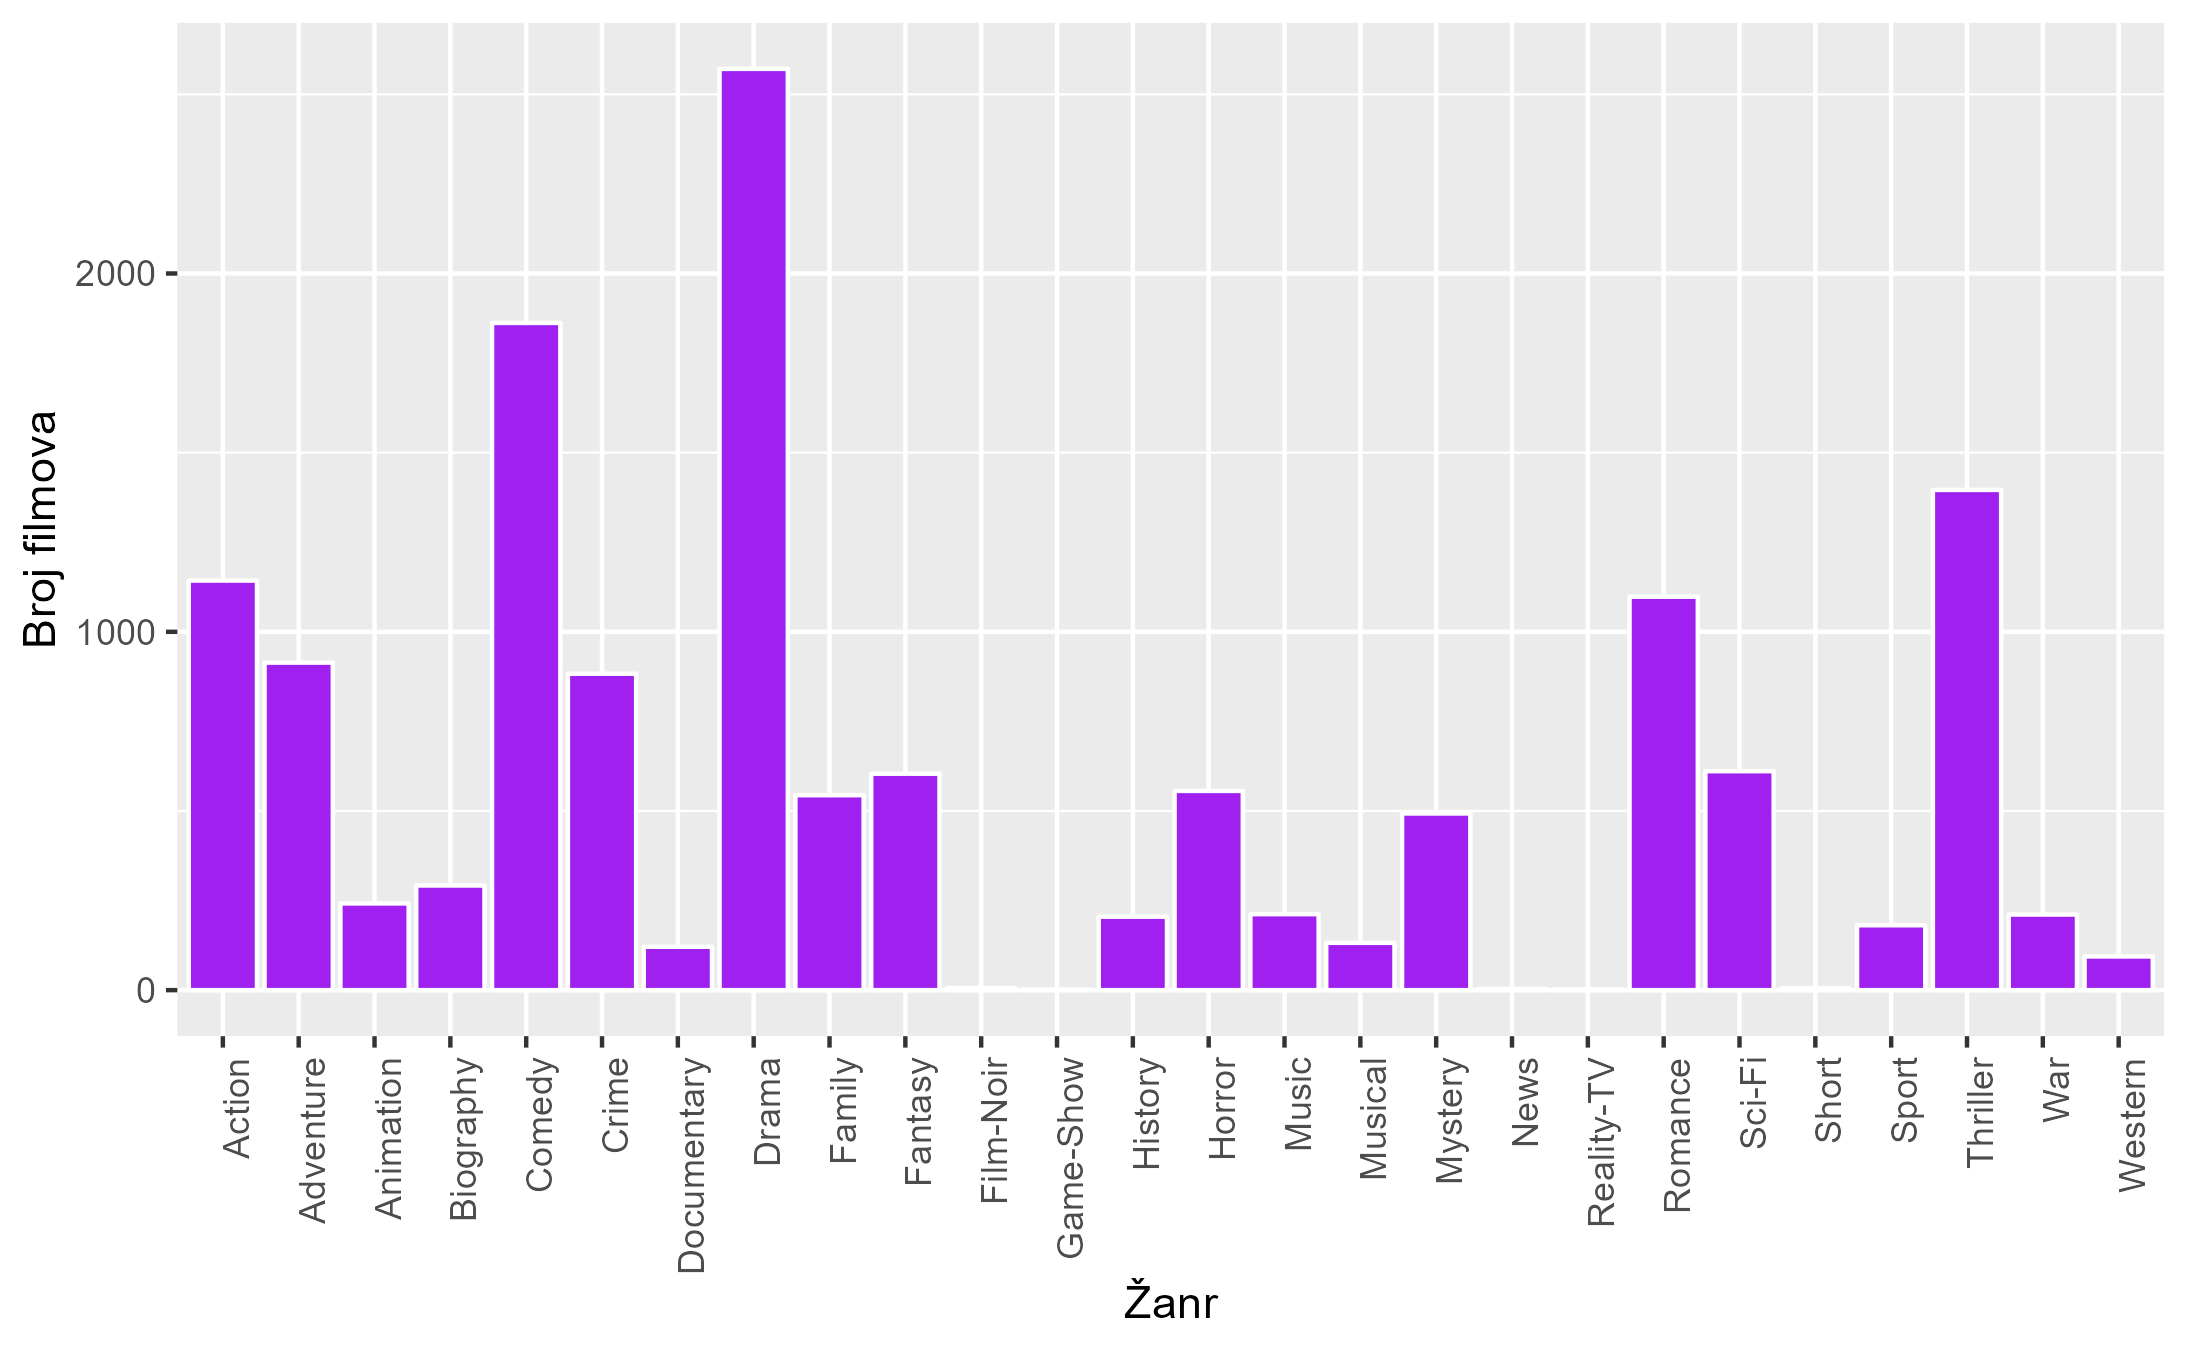
\includegraphics[width=15cm]{../figures/analysis/broj_filmova_po_zanru.png}
	 	\caption{Podjela filmova po žanru}
	 	\label{filmovi_zanr}
	 \end{figure}
	 
	 Stupac \texttt{title\_year} poprima vrijednosti od 1916 do 2016, a predstavlja godinu premijere filma. Koje je godine premijerno prikazano koliko filmova prikazano je na slici \ref{filmovi_godine}.
	 
	  \begin{figure}[H]
	 	\centering
	 	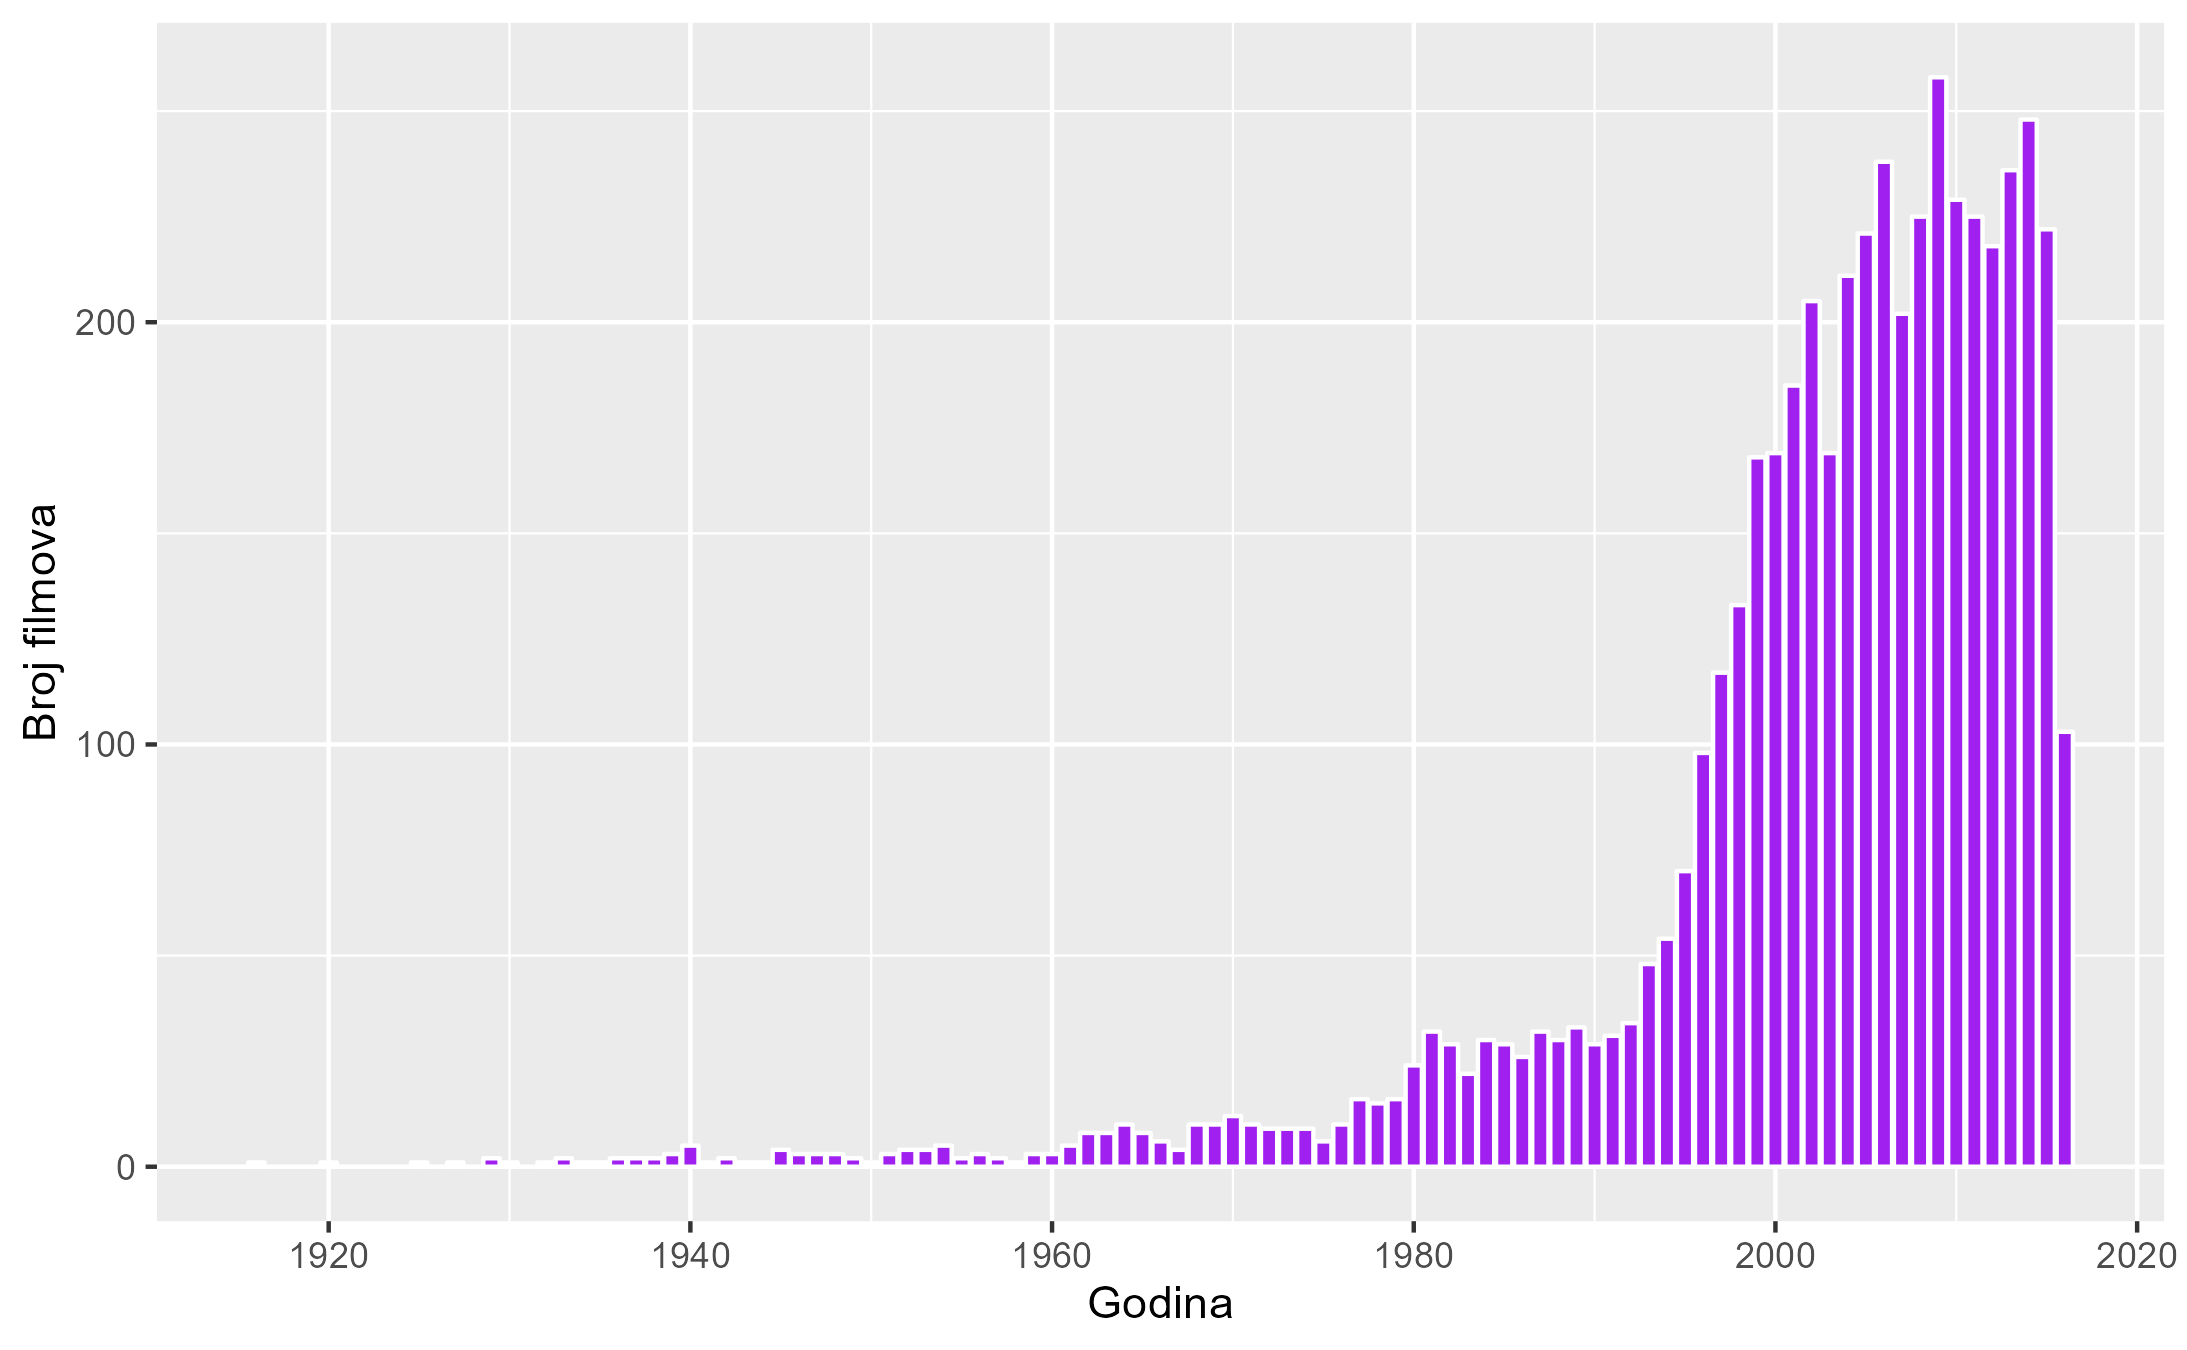
\includegraphics[width=15cm]{../figures/analysis/broj_filmova_po_godini.png}
	 	\caption{Broj filmova po godini premijere}
	 	\label{filmovi_godine}
	 \end{figure}
	 
	 U stupcu \texttt{facenumber\_in\_poster} zapisan je broj glumaca koji se pojavljuju na plakatu filma. Za većinu filmova (njih ukupno 2136) taj je broj nula, a najveći broj glumaca na plakatu iznosi 43 (za film \textit{500 Days of Summer}). Prosječna je vrijednost atributa \texttt{facenumber\_in\_poster} 1.37, a medijan 1.
	 
	 Za koju je dobnu skupinu film namijenjen sadržano je u stupcu \texttt{content\_rating}. Popis najčešćih starosnih ograničenja i njihova značenja dana su u tablici \ref{content_rating}.
	 
	 \begin{table}[H]
	 	\centering
	 	\renewcommand{\arraystretch}{1.5} % Adjust the value to increase or decrease row spacing
	 	\begin{tabular}{|c|c|l|}
	 		\hline
	 		\multicolumn{1}{|c|}{\textbf{Ograničenje}} & \multicolumn{1}{c|}{\textbf{Broj filmova}} & \multicolumn{1}{c|}{\textbf{Značenje}} \\
	 		\hline
	 		R & 2098 & Za osobe starije od 17 godina \\
	 		\hline 
	 		PG-13 & 1444 & Za osobe starije od 13 godina \\
	 		\hline
	 		PG & 688 & Za osobe starije od 8 godina \\
	 		\hline
	 	\end{tabular}
	 	\caption{Najčešća starosna ograničenja filmova}
	 	\label{content_rating}
	 \end{table}
	 
	 Omjer širine i visine (proporcije) filmske slike za pojedini film zapisan je u stupcu \texttt{aspect\_ratio}. U skupu podataka pojavljuje se ukupno 23 različitih omjera, a za sedam najčešćih napravljen je pregled (slika \ref{proporcije}) kretanja broja filmova s tim proporcijama po godinama. 
	 
	  \begin{figure}[H]
	 	\centering
	 	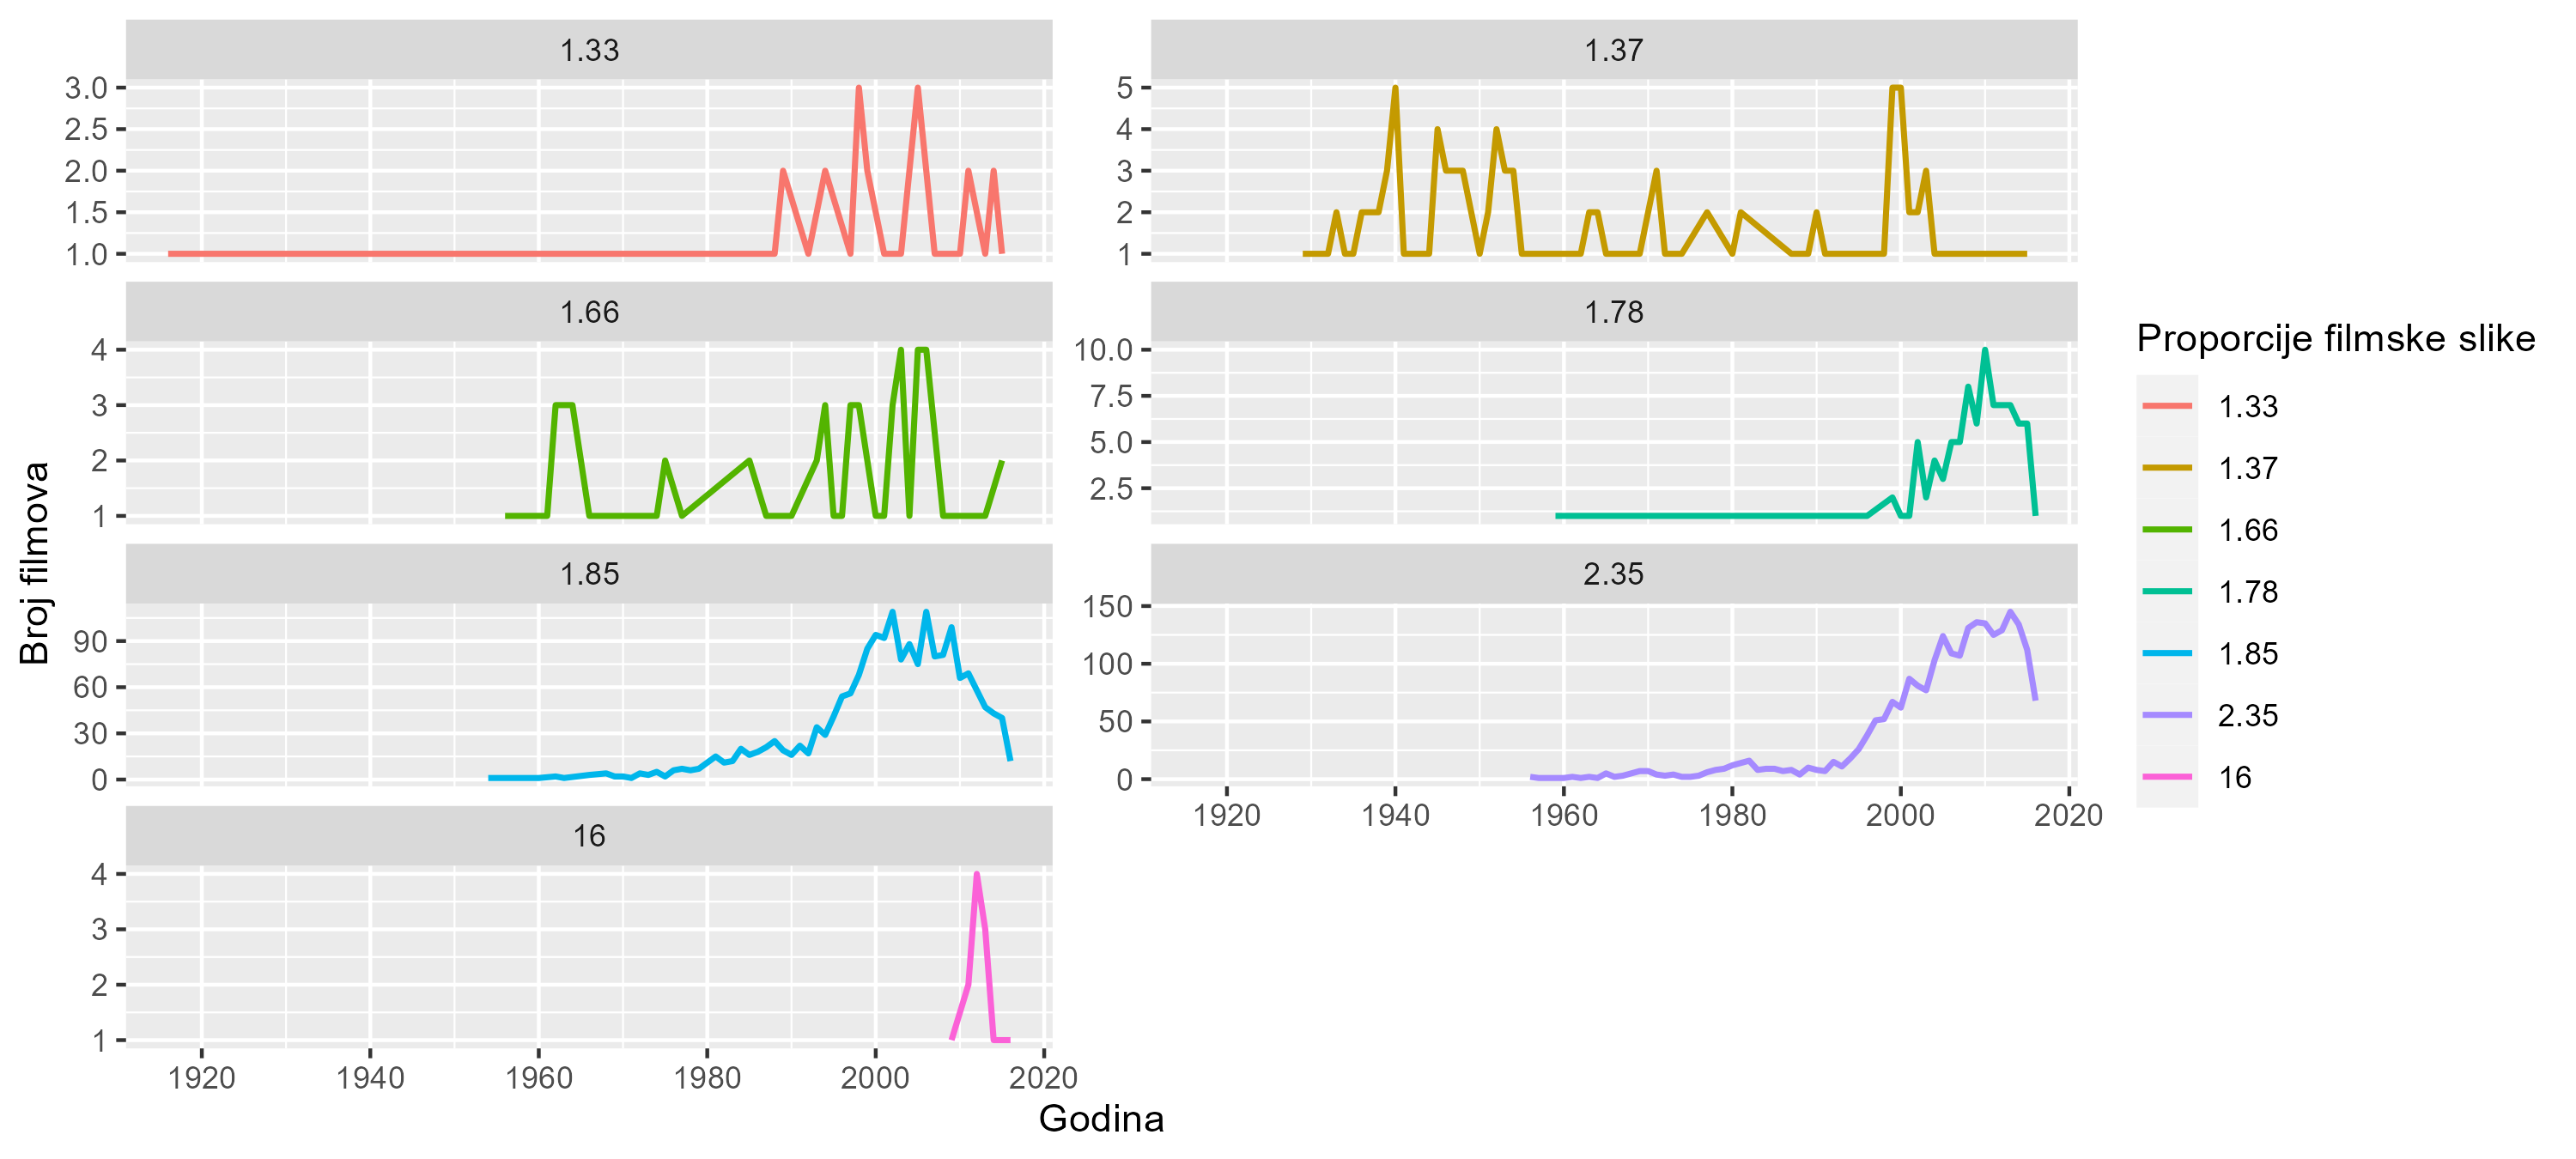
\includegraphics[width=15cm]{../figures/analysis/proporcije_i_godine.png}
	 	\caption{Broj filmova s najčešćim proporcijama filmske slike po godinama }
	 	\label{proporcije}
	 \end{figure}
	 
	 U stupcima \texttt{budget} i \texttt{gross} nalaze se podaci o budžetu filma i ukupnoj bruto zaradi filma u američkim dolarima. Koliki je postotak filmova svake godine ostvario manju zaradu od iznosa budžeta prikazujemo na slici \ref{neuspjesno}.
	 
	 
	 \begin{figure}[H]
	 	\centering
	 	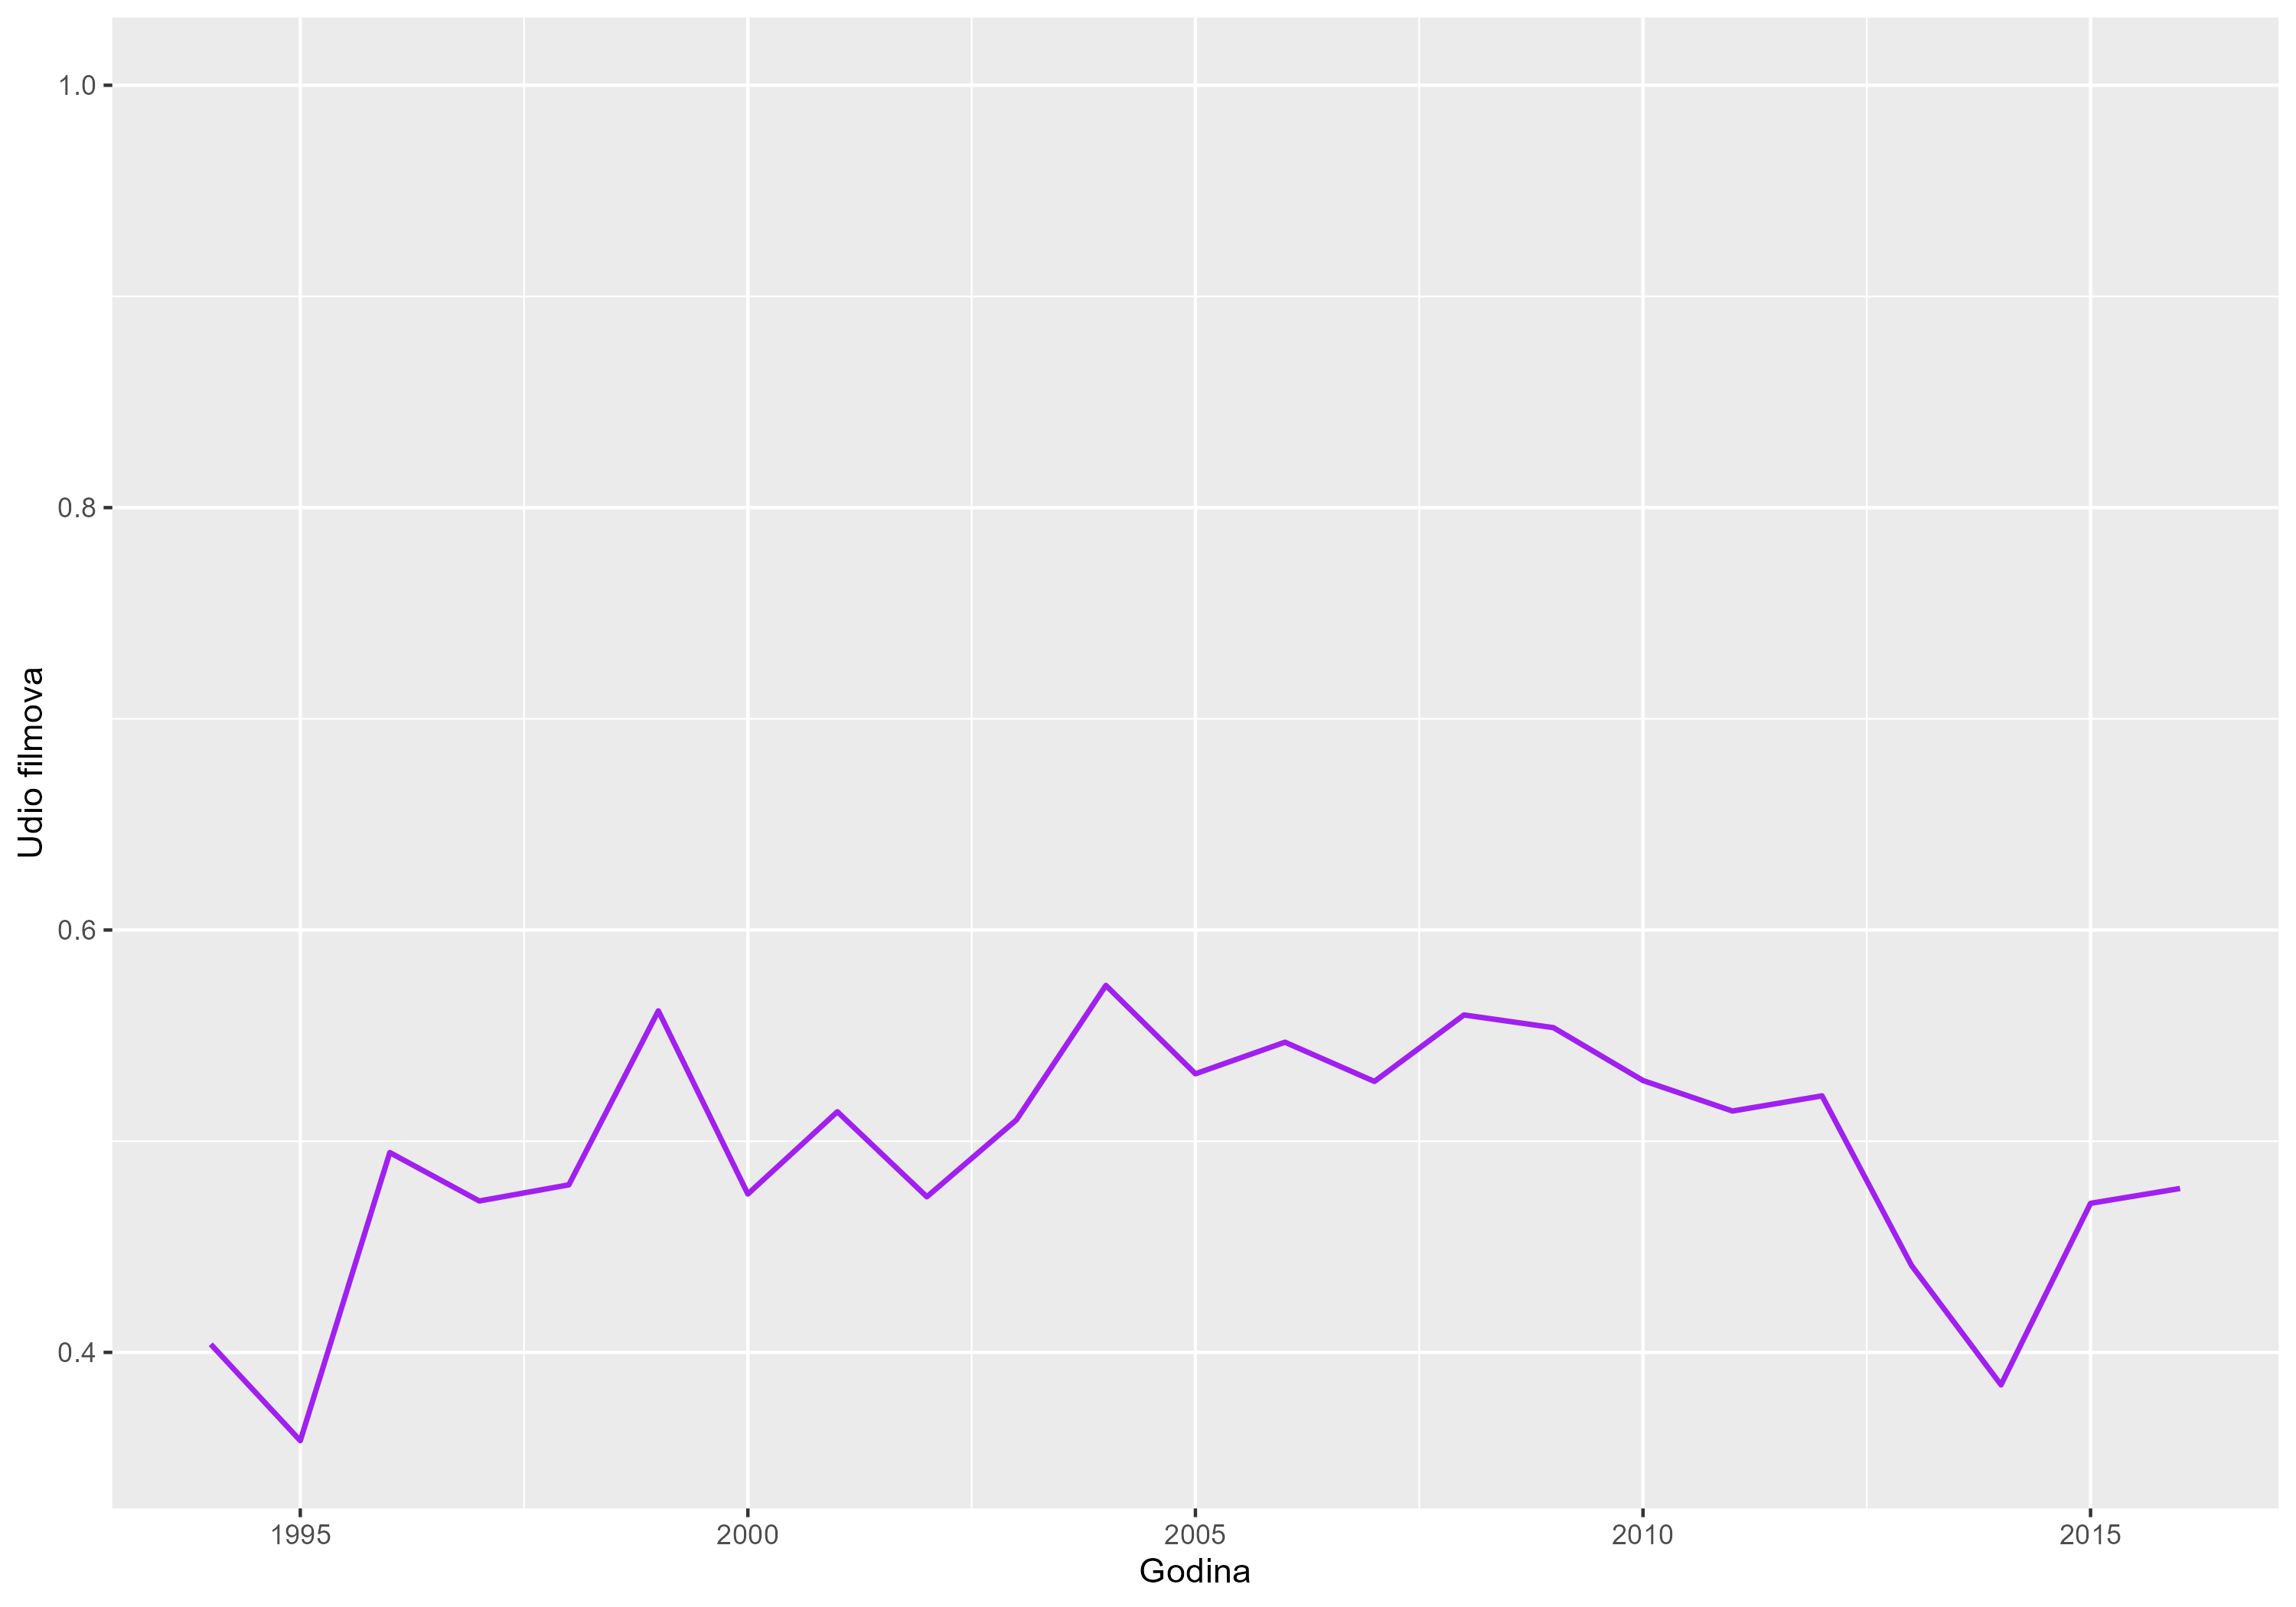
\includegraphics[width=15cm]{../figures/analysis/prihod_manji_od_budzeta.png}
	 	\caption{Postotak filmova koji su ostvarili manji prihoda od iznosa budžeta}
	 	\label{neuspjesno}
	 \end{figure}
	 
	 Stupac \texttt{duration} sadrži podatke o trajanju filmova. Najkraći film iz našeg skupa podataka traje 7, a najduži 511 minuta. Prosječno film traje 107 minuta. Histogram na slici \ref{trajanje} prikazuje broj filmova u ovisnosti o njihovom trajanju. 
	 
	  \begin{figure}[H]
	 	\centering
	 	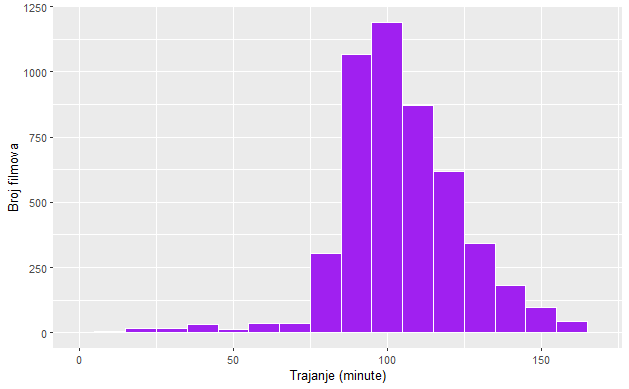
\includegraphics[width=15cm]{../figures/lucija_jednostavni/trajanje.png}
	 	\caption{Broj filmova po trajanju}
	 	\label{trajanje}
	 \end{figure}
	 
	 Većina filmova snimljena je u Sjedinjenim Američkim Državama te je na engleskom jeziku. Ipak, zastupljeno je i ponešto filmova iz drugih zemalja i na drugim jezicima. U tablicama \ref{drzava} i \ref{jezik} izdvajamo broj filmova snimljenih u najzastupljenijim državama i na najzastupljenijim jezicima. 
	 
	 \begin{table}[H]
	 	\centering
	 	\renewcommand{\arraystretch}{1.5} % Adjust the value to increase or decrease row spacing
	 	\begin{tabular}{|l|c|}
	 		\hline
	 		\multicolumn{1}{|c|}{\textbf{Država}} & \multicolumn{1}{c|}{\textbf{Broj filmova}} \\
	 		\hline
	 		SAD & 3773 \\
	 		\hline
	 		UK & 443  \\
	 		\hline
	 		Francuska & 154  \\
	 		\hline
	 		Kanada & 124  \\
	 		\hline
	 		Njemačka & 96 \\
	 		\hline
	 	\end{tabular}
	 	\caption{Podjela filmova po državi nastanka}
	 	\label{drzava}
	 \end{table} 	 
	 
	\begin{table}[H]
		\centering
		\renewcommand{\arraystretch}{1.5} % Adjust the value to increase or decrease row spacing
		\begin{tabular}{|l|c|}
			\hline
			\multicolumn{1}{|c|}{\textbf{Jezik}} & \multicolumn{1}{c|}{\textbf{Broj filmova}} \\
			\hline
			engleski & 4662 \\
			\hline
			francuski & 73  \\
			\hline
			španjolski & 40  \\
			\hline
			hindi & 28  \\
			\hline
			kineski & 24 \\
			\hline
		\end{tabular}
		\caption{Podjela filmova po jeziku}
		\label{jezik}
	\end{table} 
	 
	 Posljednji stupac, \texttt{imdb\_score}, sadrži podatak o prosječnoj ocjeni kojom su korisnici portala IMDb ocijenili pojedini film. Graf na slici \ref{imdb} prikazuje broj filmova po prosječnoj ocjeni.
	 
	 \begin{figure}[H]
	 	\centering
	 	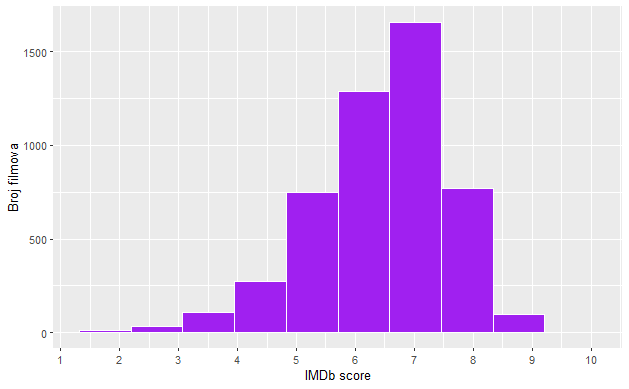
\includegraphics[width=15cm]{../figures/lucija_jednostavni/imdb.png}
	 	\caption{Podjela filmova po uspješnosti}
	 	\label{imdb}
	 \end{figure}
	
	 
	 
	 
	 
	 
	 
	 
	 
	\eject
		\chapter{Naprednije analize podataka}

	\section{Proučavanje međusobne ovisnosti atributa}
	
	\begin{figure}[H]
		\centering
		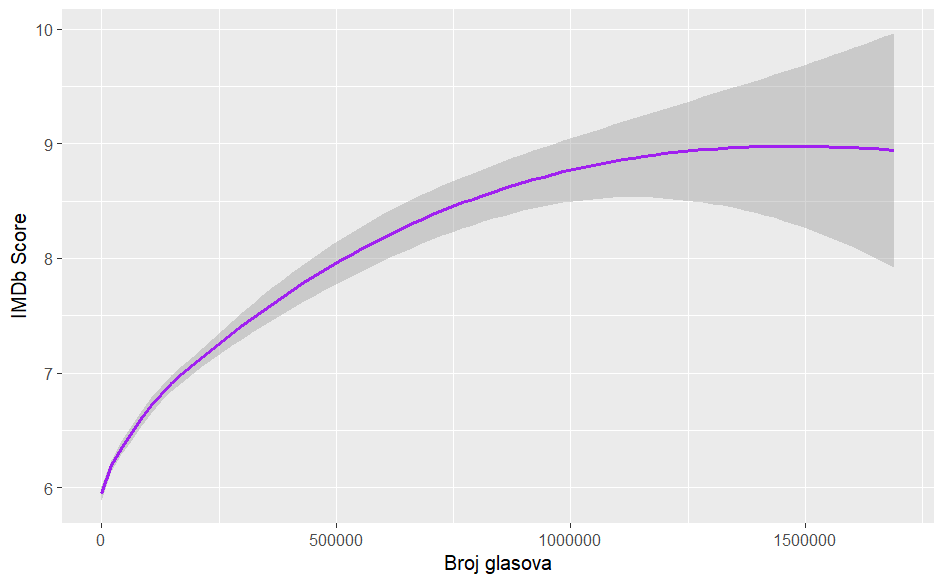
\includegraphics[width=15cm]{../figures/lucija_slozeni/glasoviocjena.png}
		\caption{IMDb ocjena u ovisnosti o broju glasova}
		\label{napredni1}
	\end{figure}
	
	\begin{figure}[H]
		\centering
		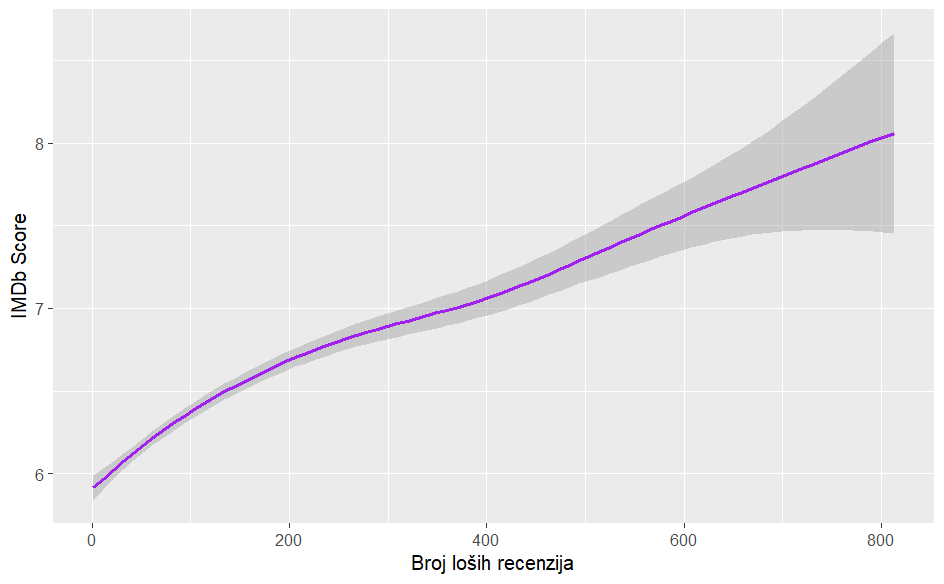
\includegraphics[width=15cm]{../figures/lucija_slozeni/loseocjena.png}
		\caption{IMDb ocjena u ovisnosti o broju loših recenzija}
		\label{napredni2}
	\end{figure}
	
	\begin{figure}[H]
		\centering
		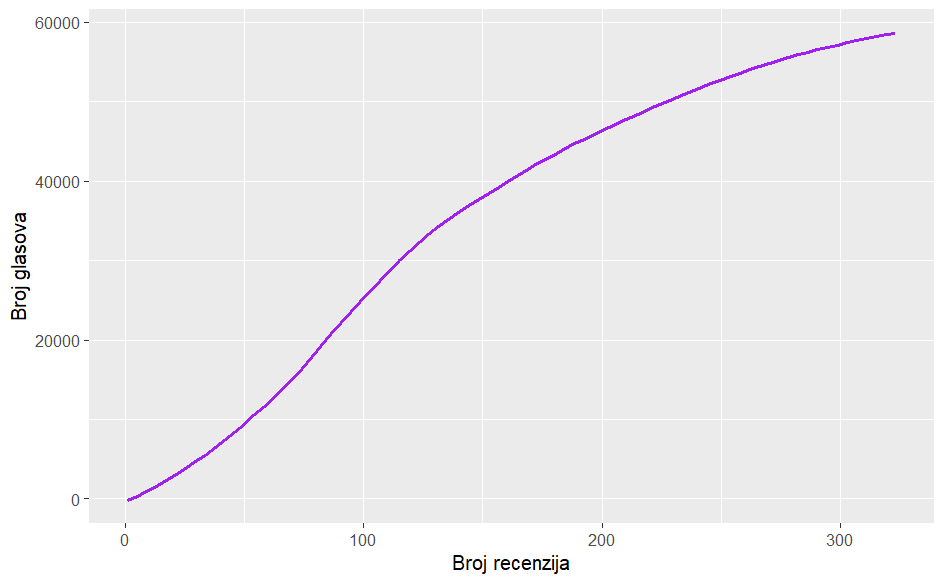
\includegraphics[width=15cm]{../figures/lucija_slozeni/recenzijeglasovi.png}
		\caption{Broj loših recenzija u ovisnosti o ukupnom broju recenzija}
		\label{napredni3}
	\end{figure}
	
	\begin{figure}[H]
		\centering
		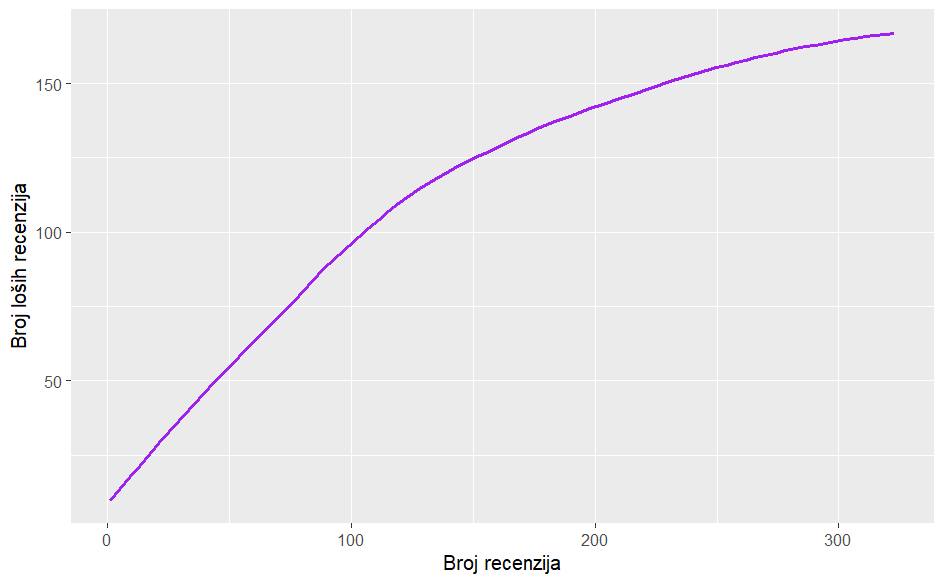
\includegraphics[width=15cm]{../figures/lucija_slozeni/recenzijelose.png}
		\caption{}
		\label{napredni4}
	\end{figure}
	
	
	\section{Dodatne zanimljive vizualizacije}
		\definecolor{codegreen}{rgb}{0,0.6,0}
\definecolor{codegray}{rgb}{0.5,0.5,0.5}
\definecolor{codepurple}{rgb}{0.58,0,0.82}
\definecolor{backcolour}{rgb}{0.95,0.95,0.92}

\lstdefinestyle{mystyle}{
	backgroundcolor=\color{backcolour},   
	commentstyle=\color{codegreen},
	keywordstyle=\color{magenta},
	numberstyle=\tiny\color{codegray},
	stringstyle=\color{codepurple},
	basicstyle=\ttfamily\footnotesize,
	breakatwhitespace=false,         
	breaklines=true,                 
	captionpos=b,                    
	keepspaces=true,                 
	numbers=left,                    
	numbersep=5pt,                  
	showspaces=false,                
	showstringspaces=false,
	showtabs=false,                  
	tabsize=2
}

\lstset{style=mystyle}


\chapter{Prediktivni modeli primjenom strojnog učenja}

Kako bismo bolje razumjeli što film čini uspješnim ili neuspješnim, provele smo analizu dobivenog skupa podataka primjenom strojnog učenja. Cilj nam je bio razviti model koji može čim točnije predviđati uspjeh filma na temelju njegovih karakteristika.
\\
\section{Priprema podataka}
Iz dobivenih podataka izbacile smo retke kojima su nedostajali neki podaci. Takvih je redaka bilo 1261. Također, uklonile smo stupce koji su sadržavali jedinstvene ili skoro jedinstvene vrijednosti (\textit{movie\_title, movie\_imdb\_link, plot\_keywords, genres}). Još smo izbacile tekstualne stupce koji su bili prekorelirani s nekim numeričkim stupcem. Na primjer, \textit{actor\_1\_name} je prekoreliran s \textit{actor\_1\_facebook\_likes}. 

\lstinputlisting[language=R]{../R/001.R} 
Preostale nenumeričke stupce pretvorile smo u tip integer. 

\lstinputlisting[language=R]{../R/002.R}

Značajka koju predviđamo je \textit{imdb\_score}. To broj zaokružen na jednu decimalu, pa smo za bolje rezultate uspjeh filma podijelile u tri skupine: loš, osrednji i dobar, a stupac imdb\_score smo zbog prekoreliranosti uklonile. 

\lstinputlisting[language=R]{../R/003.R}

Graf \ref{fig:ml1} prikazuje omjer broja filmova po uspjehu. Filmova koji su ocijenjeni kao loši znatno je manje od ostalih. Točnije, loših je filmova 43, osrednjih 1981, a dobrih 1746.

\begin{figure}
	\centering
	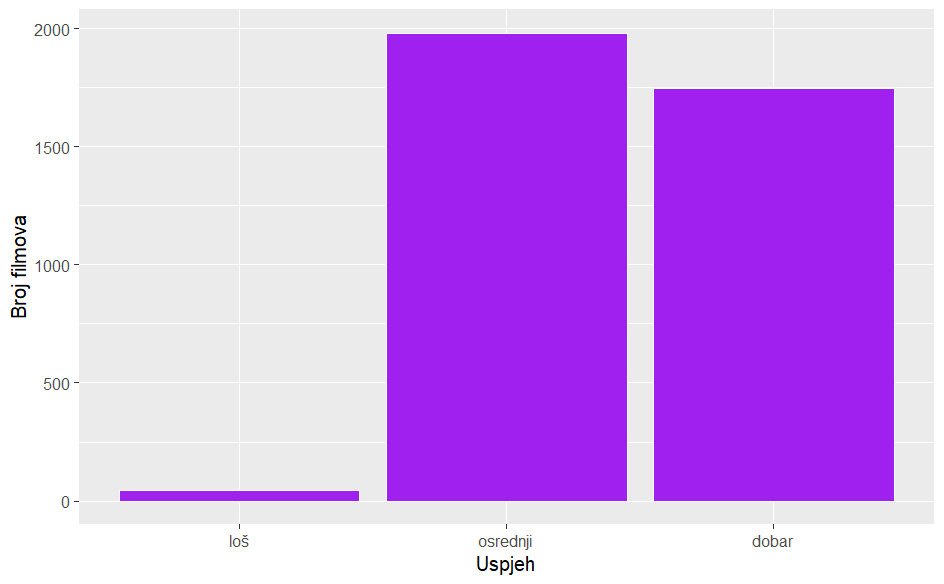
\includegraphics[width=15cm]{../figures/expl/001.png}
	\caption{Podjela filmova po uspjehu}
	\label{fig:ml1}
\end{figure}


\lstinputlisting[language=R]{../R/004.R}

\begin{center}
	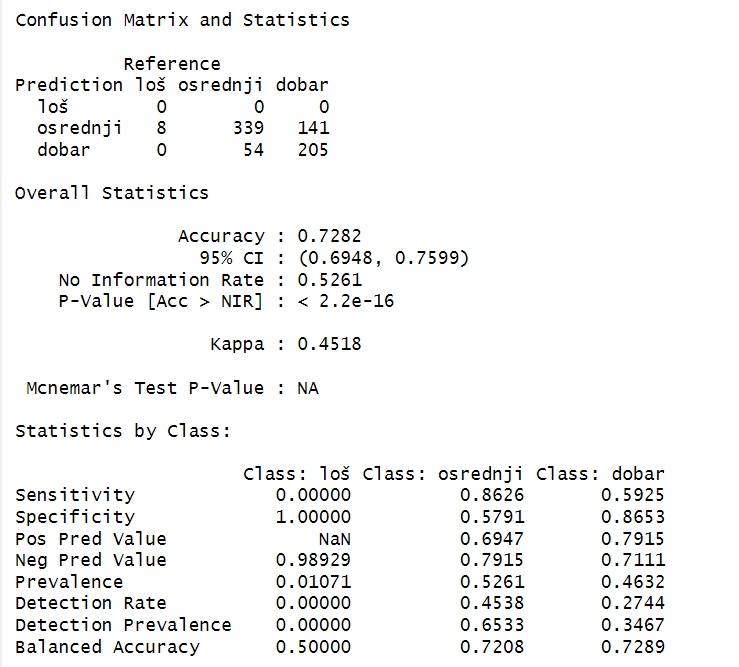
\includegraphics{../figures/expl/002.png}
\end{center}

\lstinputlisting[language=R]{../R/005.R}

\begin{center}
	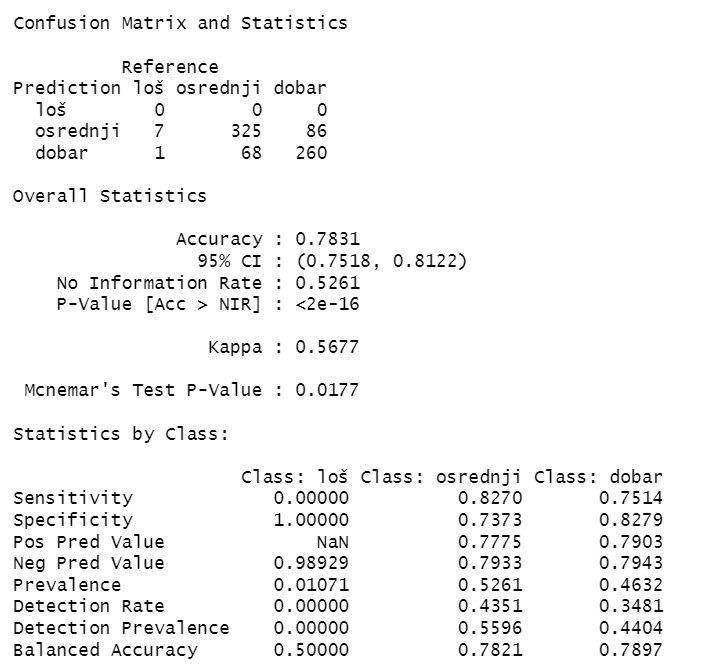
\includegraphics{../figures/expl/003.png}
\end{center}

\lstinputlisting[language=R]{../R/006.R}

\begin{center}
	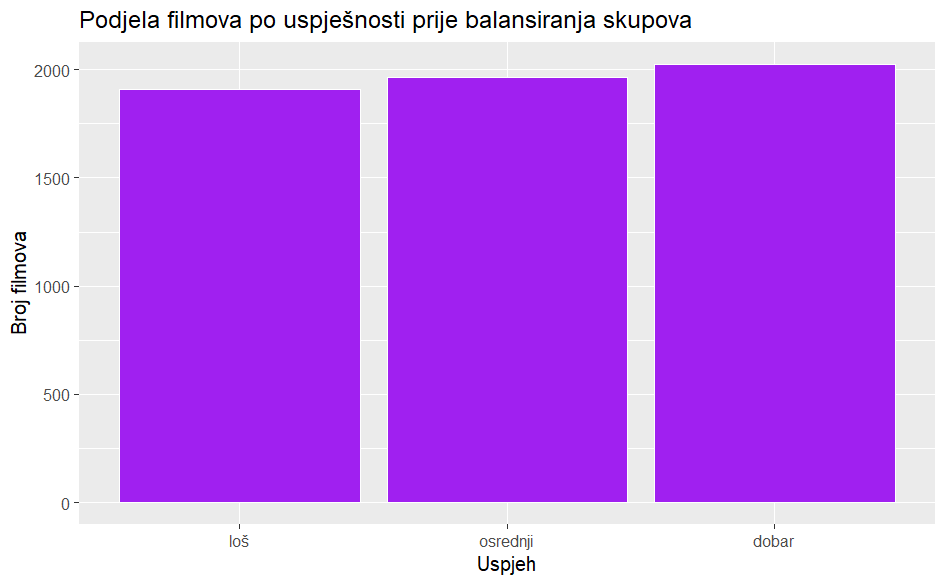
\includegraphics[width=15cm]{../figures/expl/004.png}
\end{center}

\begin{center}
	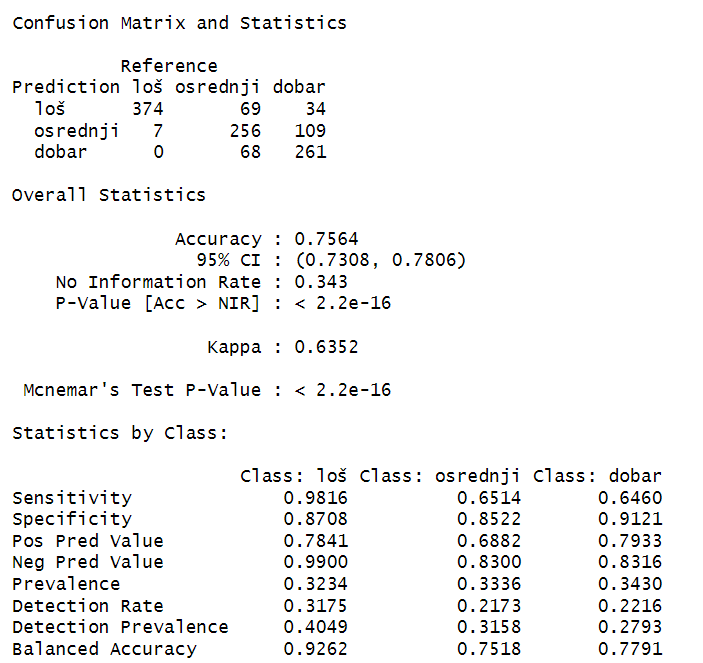
\includegraphics{../figures/expl/005.png}
\end{center}

\begin{center}
	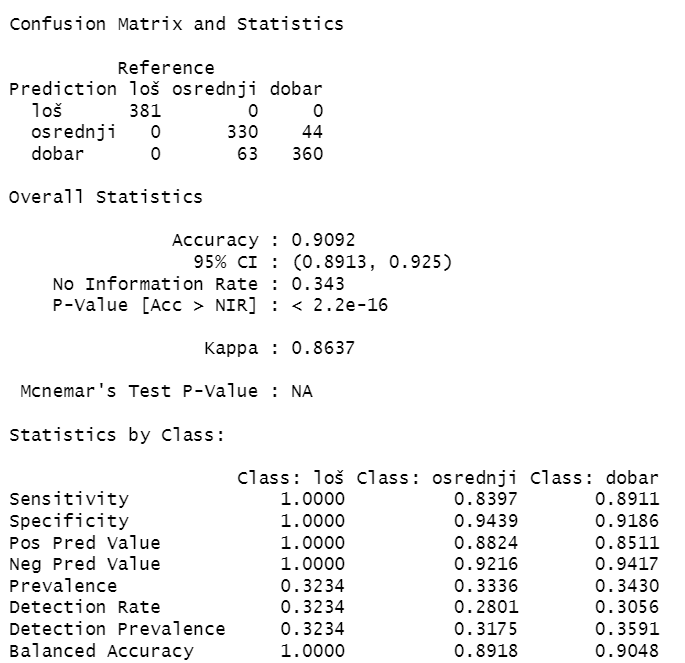
\includegraphics{../figures/expl/006.png}
\end{center}

\begin{center}
	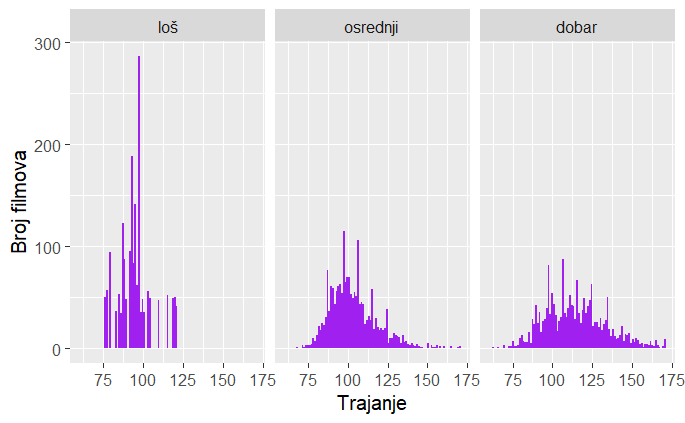
\includegraphics[width=15cm]{../figures/expl/007.png}
\end{center}

\begin{center}
	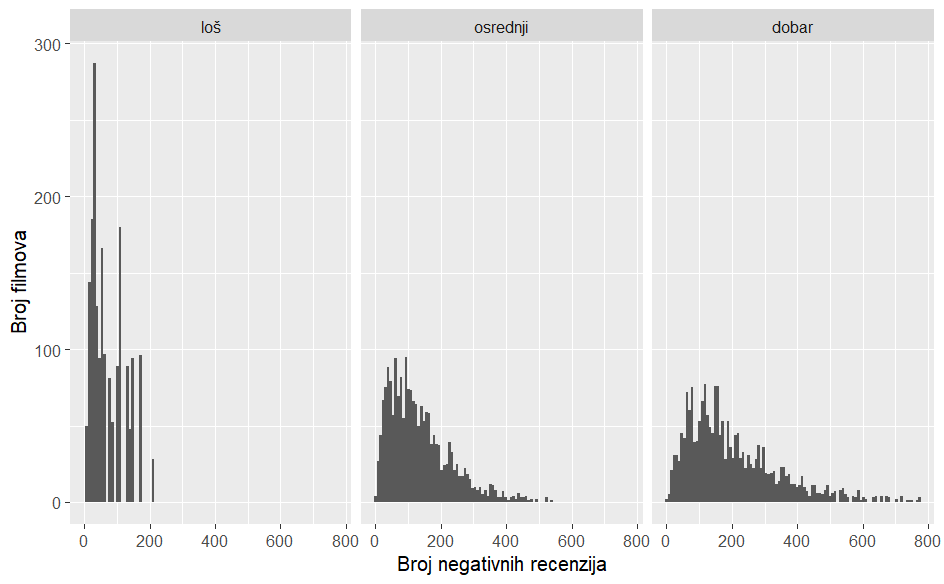
\includegraphics[width=15cm]{../figures/expl/008.png}
\end{center}


\eject
		
		
		\begingroup
		\renewcommand*\listfigurename{Indeks slika i dijagrama}
		%\renewcommand*\listtablename{Indeks tablica}
		%\let\clearpage\relax
		\listoffigures
		%\vspace{10mm}
		%\listoftables
		\endgroup
		\addcontentsline{toc}{chapter}{Indeks slika i dijagrama}
		
		
		
		\eject 
		
		
		
	\end{document} %naredbe i tekst nakon ove naredbe ne ulaze u izgrađen dokument 
	
